\documentclass[a4paper]{article}
%\usepackage{blindtext}
\usepackage{graphicx}
\usepackage{xcolor}
\usepackage[
  colorlinks = true,
  linkcolor = blue,
  urlcolor  = blue,
  citecolor = blue,
  anchorcolor = blue
              ]{hyperref}

\parindent=0pt
\begin{document}
%\textcolor{red}{\Huge Yi\u{g}it G\"und\"u\c{c}}\\
\noindent
\begin{minipage}{0.4\textwidth}
 \centering
 \fbox{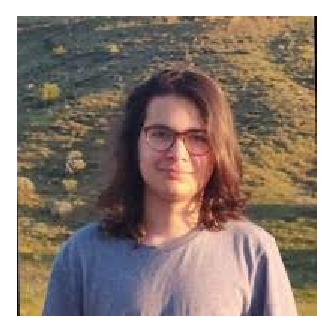
\includegraphics[scale=0.9]{yigit.eps}}
%\captionof{figure}{Caption for image}
\label{fig:sample_figure}
\end{minipage}
\hskip 0.2cm
\begin{minipage}{0.6\textwidth}
%  \vskip 0.1cm
  %\textcolor{red}{\huge Personal Info \hfill}\\
%  \textcolor{red}{\huge Yi\u{g}it G\"und\"u\c{c}}\\
%  \vskip 0.cm
%\textcolor{red}{\large e-mail :}\\
%ygunduc@gmail.com \\

%\textcolor{red}{\large git-hub :}\\
%\verb+github.com/YigitGunduc,+ \\


%\textcolor{red}{\large LinkedIn :}\\
%\verb+www.linkedin.com/in/yigit-gunduc-684131214/+ \\

\begin{tabular}{lcl}
Name           &:& \textcolor{red}{\Large Yigit} \\
Surname        &:& \textcolor{red}{\Large Gunduc} \\
Date of birth  &:& 23 Haziran 2004\\
Place of birth &:& Ankara/Turkey \\
Nationality    &:& Turkish  \\
E-mail         &:& \href{mailto:ygunduc@gmail.com}{ygunduc@gmail.com} \\
Web            &:& \href{https://github.com/YigitGunduc}{github.com/YigitGunduc}\\
               & & \url{www.linkedin.com/in/yigit-gunduc-684131214}
\end{tabular} 
\end{minipage}\\
%\end{document}
%-----------------------------------------------------------------------
\vskip 0.5cm
\textcolor{red}{\huge Education :\hfill}\\
\vskip 0.3cm
Ankara University Development Foundation Private Anatolian High School\\
Years : $2018 -$\\
(High School Grades are Documented in Appendix II:)
\begin{itemize}
\item {Cambridge International General Certificate of Secondary Education (IGCE)\\
Years:  $2018-2020$} \\
(Documented in Appendix I)
\item Cambridge International AS and A Level  (Three Subjects) \\
 Years : $2020-2021$\\
\begin{enumerate}
\item AS Level (October $2020 -$ June $2021$)
\item A2 Level (to be completed by November $2021$)
\end{enumerate}
(Documented in Appendix I)
\end{itemize}

%-----------------------------------------------------------------------
\vskip 0.5cm
\textcolor{red}{\huge Languages :\hfill}\\
\vskip 0.3cm
\begin{tabular}{lcl}
  Turkish &:& Native\\
  English &:& Very good
\end{tabular}
%-----------------------------------------------------------------------
\vskip 0.5cm
\textcolor{red}{\huge Skils    : \hfill }\\
\vskip 0.2cm
\textcolor{red}{\large Technical skils :}\\
\vskip 0.1cm
\begin{tabular}{lcl}
Programming Languages    &:& C, Python, Javascript, HTML, CSS, Latex, Dart\\
Program Packages         &:& Numpy, Flask, PyTorch, Tensorflow/Keras, Flutter
\end{tabular}
\vskip 0.2cm
\textcolor{red}{\large Soft Skils      :}\\
\vskip 0.1cm
\begin{tabular}{l}
  Critical Thinking, Problem Solving, Collaboration, Adaptibility.
\end{tabular}


%-----------------------------------------------------------------------
\vskip 0.5cm
\textcolor{red}{\huge Scientific Interests : \hfill}\\
\vskip 0.1cm
Deep Neural Networks (DNN). Natural Language Processing (NLP) , Convolutional Networks (CNN),  Generative Adversarial Networks (GANs), Computer Vision, Image Processing/recovery.  
%-----------------------------------------------------------------------
\vskip 0.5cm
\textcolor{red}{\huge Projects :\hfill }\\
\vskip 0.3cm
\hskip 1cm
\begin{minipage}{0.95\textwidth}
  \begin{description}
  \item[data-labeler]\hfill \\
    Extracts object from raw images to train machine learning or deep learning models. (\href{https://github.com/YigitGunduc/data-labeler}{https://github.com/YigitGunduc/data-labeler})
    
  \item[self-driving-car] \hfill \\
    A self-driving car that can navigate in the gta5 streets. Implemented in PyTorch. (\href{https://github.com/YigitGunduc/self-driving-car}{https://github.com/YigitGunduc/self-driving-car})
    
  \item[AIParrot] \hfill\\
    AIParrot is an intelligent conversational AI that uses machine learning to generate responses to a given question. (\href{https://github.com/YigitGunduc/AIParrot}{https://github.com/YigitGunduc/AIParrot})
    
  \item[microdb] \hfill\\
    MicroDB is open-source in memory key-value store written in C. (\href{https://github.com/YigitGunduc/microdb}{https://github.com/YigitGunduc/microdb})

  \item[Conditional-GANs-CGANs] \hfill\\
    Conditional Generative Adversarial Networks(cgans) to convert text to image implemented in Python and TensorFlow \& Keras. (\href{https://github.com/YigitGunduc/Conditional-GANs-CGANs}{https://github.com/YigitGunduc/Conditional-GANs-CGANs})
    
  \item[Spectrum] \hfill\\
    Spectrum is an AI that uses machine learning to generate Rap song lyrics. (\href{https://github.com/YigitGunduc/Spectrum}{https://github.com/YigitGunduc/Spectrum})

  \end{description}
\end{minipage}
%-----------------------------------------------------------------------
\vskip 0.5cm
\textcolor{red}{\huge Publications : \hfill}\\
\begin{enumerate}
\item SequenceGan : Text to image synthesis with Seq models and GANs\\
  Yigit Gunduc,\hfill\\
Full text from:\hfill\\
 TechRxiv. Preprint, \href{https://www.techrxiv.org/articles/preprint/SequenceGan_text_to_image_synthesis_with_Seq_models_and_GANs/14922633}{Full text from : www.techrxiv.org }\\
  \href{https://github.com/YigitGunduc/SequenceGAN}{https://github.com/YigitGunduc/SequenceGAN}

\item Tensor-to-Image: Image-to-Image Translation with Vision Transformers\\
  Yigit Gunduc,\hfill\\
  Full text from:\hfill\\
  TechRxiv. Preprint, \href{https://doi.org/10.36227/techrxiv.16727140.v1}{https://doi.org/10.36227/techrxiv.16727140.v1},\\
  \href{https://arxiv.org/pdf/2110.08037.pdf}{https://arxiv.org/pdf/2110.08037.pdf},\\
  \href{https://github.com/YigitGunduc/tensor-to-image}{https://github.com/YigitGunduc/tensor-to-image}\\
  
\item Vit-GAN: Image-to-image Translation with Vision Transformes and Conditional GANS,\\
  Yigit Gunduc,\hfill\\
  Full text from:\hfill\\
  TechRxiv. Preprint, \href{https://doi.org/10.36227/techrxiv.16785751.v1}{https://doi.org/10.36227/techrxiv.16785751.v1},\\
\href{https://arxiv.org/pdf/2110.08037.pdf}{https://arxiv.org/pdf/2110.08037.pdf}
  
\end{enumerate}

\pagebreak
%-----------------------------------------------------------------------
\vskip 0.5cm
\textcolor{red}{\huge Courses  and Certifications     :\hfill }\\
\vskip 0.3cm
\hskip 1cm
\begin{minipage}{0.95\textwidth}
\begin{description}
\item[Improving Deep Neural Networks:] \hfill \\
  {\bf Hyperparameter Tuning, Regularization and Optimization}\hfill\\
Issuing authority : Coursera - Andrew Ng, Instructor\\
Issued date : Nov 2020\\
IdentifierCredential ID : SJVKL5ARV8K9 
\item[Neural Networks and Deep Learning]\hfill\\
Issuing authority  : Coursera - Andrew Ng, Instructor\\
Issued date : Nov 2020\\
Identifier Credential ID : KJ9LZTCF8CD3
\item[Structuring Machine Learning Projects]\hfill\\
Issuing authority : Coursera - Andrew Ng, Instructor\\
Issued date: Nov 2020\\
Identifier Credential ID : 72EQBQYEXPZB
\item[Complete Tensorflow 2 and Deep Learning Bootcamp] \hfill\\
  Issuing authority : Udemy - Jose Portilla, Instructor\\
  Issued date : June 28, 2021
\item[The Complete 2020 Flutter Development Bootcamp with Dart]\hfill\\
  Issuing authority : Udemy - Dr. Angela Yu, Instructor\\
  Issued date : Aug 8, 2020
\item[The Complete Front-End Web Development Course]\hfill\\
Issuing authority : Udemy - Joseph Delgadillo and Nick Germaine, Instructors\\
Issued date : June 1, 2020
\end{description}
\end{minipage}


%-----------------------------------------------------------------------

(Appendix III - Certificates)\\
%-----------------------------------------------------------------------


\pagebreak


\textcolor{red}{\huge Appendix I :\hfill}\\
\vskip 0.2cm
\textcolor{red}{\Large Cambridge IGCSE and A Level Grades}\\
\vskip 0.5cm

\begin{enumerate}
\item {\textcolor{red}{\Large Cambridge International General Certificate of\\ Secondary Education (IGCSE)}\\

\begin{tabular}{lc}
Sylabus           &    Grades\\
Mathematics        &     A \\
Physics            &     B \\
English            &     C 
\end{tabular}
}
  
\item {\textcolor{red}{\Large Cambridge International AS and A Level}  \\

\begin{enumerate}    
\item {\textcolor{red}{\large AS Level (October 2020 - June 2021)} \\

\begin{tabular}{lc}
Sylabus           &    Grades\\
Mathematics        &      A  \\
Physics            &      A  \\
Computer Science   &      A  \\
\end{tabular}}\\

\item {\textcolor{red}{\large A2 Level (to be completed by November 2021)}\\

\begin{tabular}{lc}
Sylabus & Grades \\  
Mathematics  & \\
Physics      &  \\
Computer Science & \\
\end{tabular}
}
\end{enumerate}
  }
\end{enumerate}  


\pagebreak

\textcolor{red}{\huge Appendix II : \hfill}\\
\vskip 0.2cm
\textcolor{red}{\Large Certificates}\\
\vskip 0.5cm


\includegraphics[scale=0.06]{../Documents/out1.eps}\\

\includegraphics[scale=0.06]{../Documents/out2.eps}\\

\includegraphics[scale=0.06]{../Documents/out3.eps}


\pagebreak

\includegraphics[scale=0.05]{../Documents/UC-1.eps}\\

\includegraphics[scale=0.05]{../Documents/UC-2.eps}\\

\includegraphics[scale=0.05]{../Documents/UC-3.eps}\\


\end{document}

